\documentclass[a4paper, 14pt]{extarticle}

% Поля
%--------------------------------------
\usepackage{geometry}
\geometry{a4paper,tmargin=2cm,bmargin=2cm,lmargin=3cm,rmargin=1cm}
%--------------------------------------


%Russian-specific packages
%--------------------------------------
\usepackage[T2A]{fontenc}
\usepackage[utf8]{inputenc}
\usepackage[english, main=russian]{babel}
\usepackage{cmap}
%--------------------------------------

\usepackage{textcomp}
\usepackage{amssymb}

% Красная строка
%--------------------------------------
\usepackage{indentfirst}               
%--------------------------------------             


%Graphics
%--------------------------------------
\usepackage{graphicx}
\graphicspath{ {./images/} }
\usepackage{wrapfig}
%--------------------------------------

% Полуторный интервал
%--------------------------------------
\linespread{1.3}                    
%--------------------------------------

%Выравнивание и переносы
%--------------------------------------
% Избавляемся от переполнений
\sloppy
% Запрещаем разрыв страницы после первой строки абзаца
\clubpenalty=10000
% Запрещаем разрыв страницы после последней строки абзаца
\widowpenalty=10000
%--------------------------------------

%Списки
\usepackage{enumitem}

%Подписи
\usepackage{caption} 

%Гиперссылки
\usepackage{hyperref}

\hypersetup {
	unicode=true
}

%Рисунки
%--------------------------------------
\DeclareCaptionLabelSeparator*{emdash}{~--- }
\captionsetup[figure]{labelsep=emdash,font=onehalfspacing,position=bottom}
%--------------------------------------

\usepackage{tempora}
\usepackage{amsmath}
\usepackage[dvipsnames]{xcolor}
\usepackage{listings}
\lstset{
  belowcaptionskip=1\baselineskip,
  breaklines=true,
  frame=L,
  xleftmargin=\parindent,
  language=Java,
  showstringspaces=false,
  basicstyle=\footnotesize\ttfamily,
  keywordstyle=\bfseries\color{blue},
  commentstyle=\itshape\color{purple},
  identifierstyle=\color{black},
  stringstyle=\color{red},
  numbers=left,           
  numberstyle=\tiny\color{gray}, 
  numbersep=10pt,      
  % ------------------------------
}

%--------------------------------------
%			НАЧАЛО ДОКУМЕНТА
%--------------------------------------

\begin{document}

%--------------------------------------
%			ТИТУЛЬНЫЙ ЛИСТ
%--------------------------------------
\begin{titlepage}
\thispagestyle{empty}
\newpage


%Шапка титульного листа
%--------------------------------------
\vspace*{-60pt}
\hspace{-65pt}
\begin{minipage}{0.3\textwidth}
\hspace*{-20pt}\centering

\includegraphics[width=\textwidth]{emblem}
\end{minipage}
\begin{minipage}{0.67\textwidth}\small \textbf{
\vspace*{-0.7ex}
\hspace*{-6pt}\centerline{Министерство науки и высшего образования Российской Федерации}
\vspace*{-0.7ex}
\centerline{Федеральное государственное бюджетное образовательное учреждение }
\vspace*{-0.7ex}
\centerline{высшего образования}
\vspace*{-0.7ex}
\centerline{<<Московский государственный технический университет}
\vspace*{-0.7ex}
\centerline{имени Н.Э. Баумана}
\vspace*{-0.7ex}
\centerline{(национальный исследовательский университет)>>}
\vspace*{-0.7ex}
\centerline{(МГТУ им. Н.Э. Баумана)}}
\end{minipage}
%--------------------------------------

%Полосы
%--------------------------------------
\vspace{-25pt}
\hspace{-35pt}\rule{\textwidth}{2.3pt}

\vspace*{-20.3pt}
\hspace{-35pt}\rule{\textwidth}{0.4pt}
%--------------------------------------

\vspace{1.5ex}
\hspace{-35pt} \noindent \small ФАКУЛЬТЕТ\hspace{80pt} <<Информатика и системы управления>>

\vspace*{-16pt}
\hspace{47pt}\rule{0.83\textwidth}{0.4pt}

\vspace{0.5ex}
\hspace{-35pt} \noindent \small КАФЕДРА\hspace{50pt} <<Теоретическая информатика и компьютерные технологии>>

\vspace*{-16pt}
\hspace{30pt}\rule{0.866\textwidth}{0.4pt}
  
\vspace{11em}

\begin{center}
\Large {\bf Лабораторная работа № 11} \\ 
\large {\bf по курсу <<Языки и методы программирования>>} \\ 
\large <<Разработка парсеров на языке Java>>
\end{center}\normalsize

\vspace{8em}


\begin{flushright}
  {Студент группы ИУ9-21Б Воронков А. С.\hspace*{15pt} \\
  \vspace{2ex}
  Преподаватель Посевин Д. П.\hspace*{15pt}}
\end{flushright}

\bigskip

\vfill
 

\begin{center}
\textsl{Москва 2026}
\end{center}
\end{titlepage}
%--------------------------------------
%		КОНЕЦ ТИТУЛЬНОГО ЛИСТА
%--------------------------------------

\renewcommand{\ttdefault}{pcr}

\setlength{\tabcolsep}{3pt}
\newpage
\setcounter{page}{2}

\section{Цель}\label{Sect::task}
\par 
Овладение методом рекурсивного спуска для разработки парсеров по грамматике некоторого формального языка.
Java.    
\section{Задание}
В ходе лабораторной работы нужно разработать программу, выполняющую синтаксический анализ текста по одной из LL(1)-грамматик, БНФ которых приведены в таблицах 1–6. Текст может содержать символы перевода строки.
	В записи БНФ терминальные символы IDENT, NUMBER и STRING означают идентификаторы, числа и строки, соответственно. Идентификатор – это последовательность букв и цифр, начинающаяся с буквы. Число – это непустая последовательность десятичных цифр. Строка – это обрамлённая кавычками произвольная последовательность символов, не содержащая кавычек и символов перевода строки.
	Программа должна выводить в стандартный поток вывода последовательность правил
грамматики, применение которых даёт левый вывод введённого из стандартного потока ввода текста. Если вывод не может быть построен, программа должна выводить сообщение «syntax error at (line, col)», где line и col – координаты ошибки в тексте.

<Chain> ::= IDENT <Tail> \par
<Tail>::= . IDENT ( <Arg> ) <Tail> \par
| 
e \par
<Arg>::= NUMBER | STRING | <Chain>


\pagebreak
\section{Практическая реализация}
\par
Код файла Token.java
\begin{lstlisting}
public enum Token {
    LPAREN, RPAREN, NUM, STRING, IDENT, POINT, END
}
\end{lstlisting}
\par
Код файла Tree.java
\begin{lstlisting}
import java.util.Arrays;
import java.util.List;
import java.io.PrintStream;

public class Tree {
    String node;
    List<Tree> children;

    public Tree(String node,  Tree... children) {
        this.node = node;
        this.children = Arrays.asList(children);
    }

    public Tree(String node) {
        this.node = node;
        this.children = Arrays.asList();
    }

    public void print(PrintStream out, String prefix, boolean isTail) {
        out.println(prefix + (isTail ? "└── " : "├── ") + node);
        for (int i = 0; i < children.size() - 1; i++) {
            children.get(i).print(out, prefix + (isTail ? "    " : "│   "), false);
        }
        if (children.size() > 0) {
            children.get(children.size() - 1)
                    .print(out, prefix + (isTail ? "    " : "│   "), true);
        }
    }
}
\end{lstlisting}
\par
Код файла Lexer.java
\begin{lstlisting}
import java.io.IOException ;
import java.io.InputStream ;
import java.text.ParseException ;

public class Lexer {
    InputStream is;
    int curChar;
    int curPos;
    Token curToken;
    String curStr = "";

    public Lexer(InputStream is) throws ParseException {
        this.is = is;
        curPos = 0;
        nextChar();
    }

    private boolean isBlank(int c) {
        return c == ' ' || c == '\r' || c == '\n' || c == '\t';
    }

    private void nextChar() throws ParseException {
        curPos++;
        try {
            curChar = is.read();
        } catch (IOException e) {
            throw new ParseException(e.getMessage(), curPos);
        }
    }

    public void nextToken() throws ParseException {
        while (isBlank(curChar)) {
            nextChar();
        }
        switch (curChar) {
            case '(':
                nextChar();
                curToken = Token.LPAREN;
                break;
            case ')':
                nextChar();
                curToken = Token.RPAREN;
                break;
            case '.':
                nextChar();
                curToken = Token.POINT;
                break;
            case '"':
                nextChar();
                curStr = "";
                while (curChar != '"') {
                    if (curChar == -1 || curChar == '\n' || curChar == '\r') {
                        throw new ParseException("string without end", curPos);
                    }
                    curStr += (char) curChar;
                    nextChar();
                }
                nextChar();
                curToken = Token.STRING;
                break;
            case -1:
                curToken = Token.END;
                break;
            default:
                if (Character.isDigit(curChar)) {
                    curStr = "";
                    while (Character.isDigit(curChar)) {
                        curStr += (char) curChar;
                        nextChar();
                    }
                    curToken = Token.NUM;
                } else if (Character.isAlphabetic(curChar)) {
                        curStr = "";
                    while (Character.isAlphabetic(curChar) || Character.isDigit(curChar)) {
                            curStr += (char) curChar;
                            nextChar();
                        }
                        curToken = Token.IDENT;
                } else{
                    throw new ParseException("notKnown char" + (char) curChar, curPos);
                }
                break;
        }
    }

    public Token curToken() {return curToken;}
    public int curPos() {return curPos;}
    public String curStr() { return curStr; }
}
\end{lstlisting}
\par
Код файла Parser.java
\begin{lstlisting}
import java.io.InputStream ;
import java.text.ParseException;

public class Parser {
    Lexer lex;

    Tree Chain() throws ParseException {
        if (lex.curToken == Token.IDENT) {
            String ident = lex.curStr;
            lex.nextToken();
            return new Tree("<Chain>", new Tree(ident), Tail());
        } else {
                throw new ParseException("syntax error at pos " + lex.curPos, lex.curPos);
        }
    }

    Tree Tail() throws ParseException {
        switch (lex.curToken) {
            case POINT:
                lex.nextToken();
                if (lex.curToken != Token.IDENT) {
                    throw new ParseException("syntax error at pos " + lex.curPos, lex.curPos);
                }
                String ident = lex.curStr;
                lex.nextToken();
                if (lex.curToken != Token.LPAREN) {
                    throw new ParseException("syntax error at pos " + lex.curPos, lex.curPos);
                }
                lex.nextToken();
                Tree sup = Arg();
                if (lex.curToken != Token.RPAREN) {
                    throw new ParseException("syntax error at pos " + lex.curPos, lex.curPos);
                }
                lex.nextToken();
                Tree sup2 = Tail();
                return new Tree("<Tail>", new Tree("."),
                        new Tree(ident), new Tree("("), sup, new Tree(")"), sup2);
            case RPAREN:
                case END:
                return new Tree("<Tail>");
            default:
                throw new ParseException("syntax error at pos " + lex.curPos,  lex.curPos);
        }
    }
    Tree Arg() throws ParseException {
        switch (lex.curToken) {
            case STRING:
            case NUM:
                String curStr = lex.curStr;
                lex.nextToken();
                return new Tree("<Arg>", new Tree(curStr));
            case IDENT:
                return new Tree("<Arg>", Chain());
            default:
                throw new ParseException("syntax error at pos " + lex.curPos, lex.curPos);
        }
    }

    Tree parse(InputStream is) throws ParseException {
        lex = new Lexer(is);
        lex.nextToken();

        return Chain();
    }
}
\end{lstlisting}
\par
Код файла Main.java
\begin{lstlisting}
import java.io.*;
import java.text.ParseException;

public class Main {
    public static void main(String[] args) {
        Parser parser = new Parser();
        try {
            InputStream is = new ByteArrayInputStream("a.mul(3).sub(b.div(c))".getBytes());
            Tree root = parser.parse(is);

            ByteArrayOutputStream baos = new ByteArrayOutputStream();
            PrintStream ps = new PrintStream(baos, true, "UTF-8");
            root.print(ps, "", true);

            System.out.println(baos.toString("UTF-8"));
        } catch (ParseException e) {
            System.out.println(e.getMessage());
        } catch (UnsupportedEncodingException e) {
            System.out.println("Encoding error: " + e.getMessage());
        }
    }
}
\end{lstlisting}
\par
Код файла Publisher.java
\begin{lstlisting}
import org.eclipse.paho.client.mqttv3.*;
import java.util.Scanner;


public class Publisher {
    private MqttClient client;
    private String topic = "IU/9/voronkov";

    public Publisher() throws MqttException {
        String broker = "tcp://broker.emqx.io:1883";
        String clientId = "voronkov_publisher";
        client = new MqttClient(broker, clientId);
        client.connect();
    }
    public void sendMessage(String text) {
        try{
            client.publish(topic, new MqttMessage(text.getBytes()));
        } catch (MqttException e) {
            e.printStackTrace();
        }
    }
}
\end{lstlisting}
\par
Код файла Subscriber.java
\begin{lstlisting}
import org.eclipse.paho.client.mqttv3.*;
import javax.swing.*;
import java.io.ByteArrayOutputStream;
import java.io.InputStream;
import java.io.PrintStream;


public class Subscriber {
    private MqttClient client;
    private String topic = "IU/9/voronkov";
    private PictureForm gui;

    public Subscriber(PictureForm gui  ) throws MqttException{
        String broker = "tcp://broker.emqx.io:1883";
        String clientId = "voronkov_subscriber";
        try {
            this.client = new MqttClient(broker, clientId);
            MqttConnectOptions opts = new MqttConnectOptions();

            client.setCallback(new MqttCallback() {
                public void messageArrived(String topic, MqttMessage message) throws Exception {
                    String mes = new String(message.getPayload());
                    System.out.println("message content: " + mes);
                    try {
                        InputStream body = new java.io.ByteArrayInputStream(mes.getBytes());
                        Parser parser = new Parser();
                        Tree tree = parser.parse(body);

                        ByteArrayOutputStream baos = new ByteArrayOutputStream();
                        PrintStream ps = new PrintStream(baos, true, "UTF-8");
                        tree.print(ps, "", true);
                        String result = baos.toString("UTF-8");
                        SwingUtilities.invokeLater(() -> {
                            gui.updateLog(result);
                        });

                    } catch (Exception e) {
                        SwingUtilities.invokeLater(() -> {
                            gui.appendMessage("Error: " + e.getMessage());
                        });
                    }
                }

                public void connectionLost(Throwable cause) {
                    System.out.println("connectionLost: " + cause.getMessage());
                }

                public void deliveryComplete(IMqttDeliveryToken token) {
                    System.out.println("deliveryComplete: " + token.isComplete());
                }
            });

            System.out.println("Connecting to broker...");
            client.connect(opts);

            client.subscribe(topic);
            System.out.println("waiting");
        } catch (MqttException e) {
            System.err.println("Error MQTT: " + e.getMessage());
            e.printStackTrace();
        }
    }
}
\end{lstlisting}
\par
Код файла PictureForm.java
\begin{lstlisting}
import org.eclipse.paho.client.mqttv3.MqttException;

import javax.swing.*;
import java.awt.*;

public class PictureForm {
    private JPanel mainPanel;
    private JTextArea textArea;
    private Publisher publisher;
    private JTextArea chatArea;
    private JTextField inputField;
    private JButton sendButton;
    public void updateLog(String text) {
        appendMessage(text);
    }

    public PictureForm(Publisher publisher) {
        JFrame frame = new JFrame("Parser");
        this.publisher = publisher;
        chatArea = new JTextArea();
        chatArea.setEditable(false);
        chatArea.setLineWrap(true);
        chatArea.setWrapStyleWord(true);
        JScrollPane scroll = new JScrollPane(chatArea);
        scroll.setPreferredSize(new Dimension(450, 350));

        inputField = new JTextField();
        inputField.addActionListener(e -> sendMessage());

        sendButton = new JButton("Отправить");
        sendButton.addActionListener(e -> sendMessage());

        JPanel bottomPanel = new JPanel(new BorderLayout());
        bottomPanel.add(inputField, BorderLayout.CENTER);
        bottomPanel.add(sendButton, BorderLayout.EAST);

        frame.setLayout(new BorderLayout());
        frame.add(scroll, BorderLayout.CENTER);
        frame.add(bottomPanel, BorderLayout.SOUTH);

        frame.setDefaultCloseOperation(JFrame.EXIT_ON_CLOSE);
        frame.pack();
        frame.setLocationRelativeTo(null);
        frame.setVisible(true);
    }

    private void sendMessage() {
        String text = inputField.getText().trim();
        if (!text.isEmpty()) {
            publisher.sendMessage(text);
            appendMessage("Result: " + text);
            inputField.setText("");
        }
    }

    public void appendMessage(String message) {
        SwingUtilities.invokeLater(() -> {
            chatArea.append(message + "\n");
            chatArea.setCaretPosition(chatArea.getDocument().getLength());
        });
    }

    public static void main(String[] args) {
        try {
            Publisher pub = new Publisher();
            PictureForm form = new PictureForm(pub);
            new Subscriber(form);
        } catch (MqttException e) {
            e.printStackTrace();
        }
    }
}
\end{lstlisting}
\par
Код файла Http.java
\begin{lstlisting}
import com.sun.net.httpserver.HttpExchange;
import com.sun.net.httpserver.HttpHandler;
import com.sun.net.httpserver.HttpServer;
import java.io.*;
import java.net.InetSocketAddress;
import java.text.ParseException;


public class Http {
    public static void main(String[] args) throws IOException {
        HttpServer server = HttpServer.create(new InetSocketAddress(5678), 0);
        server.createContext("/lab11", new MyHandlerLab11());
        server.setExecutor(null);
        server.start();
    }

    static class MyHandlerLab11 implements HttpHandler {
        @Override
        public void handle(HttpExchange exchange) throws IOException {
            if (!"POST".equals(exchange.getRequestMethod())) {
                exchange.sendResponseHeaders(405, -1);
                return;
            }

            InputStream body = exchange.getRequestBody();
            String response;
            exchange.getResponseHeaders().set("Access-Control-Allow-Origin", "*");

            try {
                Parser parser = new Parser();
                Tree tree = parser.parse(body);

                ByteArrayOutputStream baos = new ByteArrayOutputStream();
                PrintStream ps = new PrintStream(baos, true, "UTF-8");
                tree.print(ps, "", true);
                response = baos.toString("UTF-8");

            } catch (ParseException e) {
                response = e.getMessage();
            }

            byte[] bytes = response.getBytes("UTF-8");
            exchange.getResponseHeaders().set("Content-Type", "text/plain; charset=utf-8");
            exchange.sendResponseHeaders(200, bytes.length);
            OutputStream os = exchange.getResponseBody();
            os.write(bytes);
            os.close();
        }
    }
}
\end{lstlisting}
\par
Код файла index.html
\begin{lstlisting}
    <!DOCTYPE html>
<html>
<body>
<textarea id="input" rows="5" cols="40"></textarea>
<br>
<button onclick="send()">Send</button>
<pre id="output"></pre>

<script>
    async function send() {
        const text = document.getElementById("input").value;
        const res = await fetch("http://localhost:5678/lab11", {
            method: "POST",
            body: text
        });
        document.getElementById("output").textContent = await res.text();
    }
</script>
</body>
</html>
\end{lstlisting}

\section{Результаты}
В результате лабораторной работы был разработан парсер и в дополнение к нему GUI интерфейс и взаимодействие через сайт

\begin{center}
    \nopagebreak
    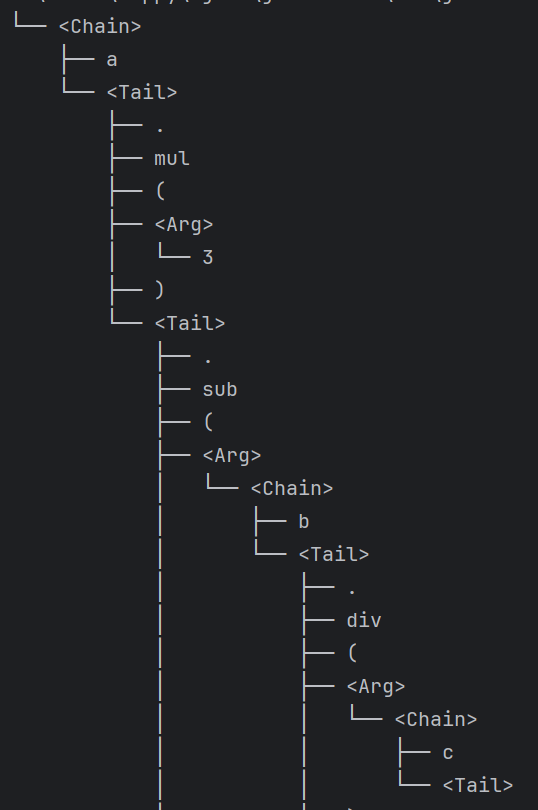
\includegraphics[width=0.85\textwidth]{lab11_1}
    \captionsetup{justification=centering}
    \captionof{figure}{Результат работы парсера}
    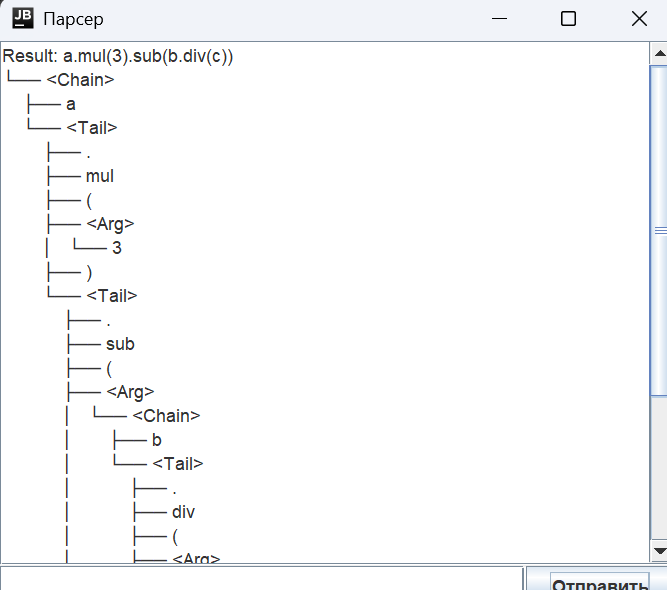
\includegraphics[width=0.85\textwidth]{lab11_2}
    \captionsetup{justification=centering}
    \captionof{figure}{Результат работы GUI}
    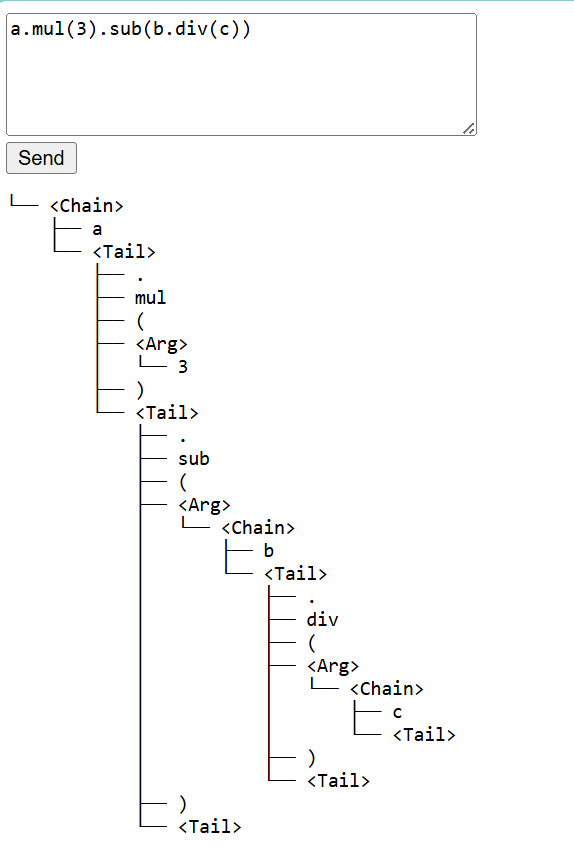
\includegraphics[width=0.85\textwidth]{lab11_3}
    \captionsetup{justification=centering}
    \captionof{figure}{Реззультат работы сайта}
\end{center}

\section{Вывод}
В данной лабораторной работе были получен навык разработки парсера через реукурсивный спуск
\end{document}